\documentclass{standalone}
\usepackage{amsmath,amssymb}
\usepackage[dvipsnames]{xcolor}
\usepackage{tikz} 
\usetikzlibrary{arrows, decorations.markings,decorations.pathreplacing,angles,quotes}
\usepackage{microtype}
\usepackage{fourier}

\definecolor{nb}{RGB}{31,119,180}


%include other needed packages here   
\begin{document}

\begin{tikzpicture}
% include your tikz code here
    		\node[anchor=south west,inner sep=0] (Bild) at (0,0) {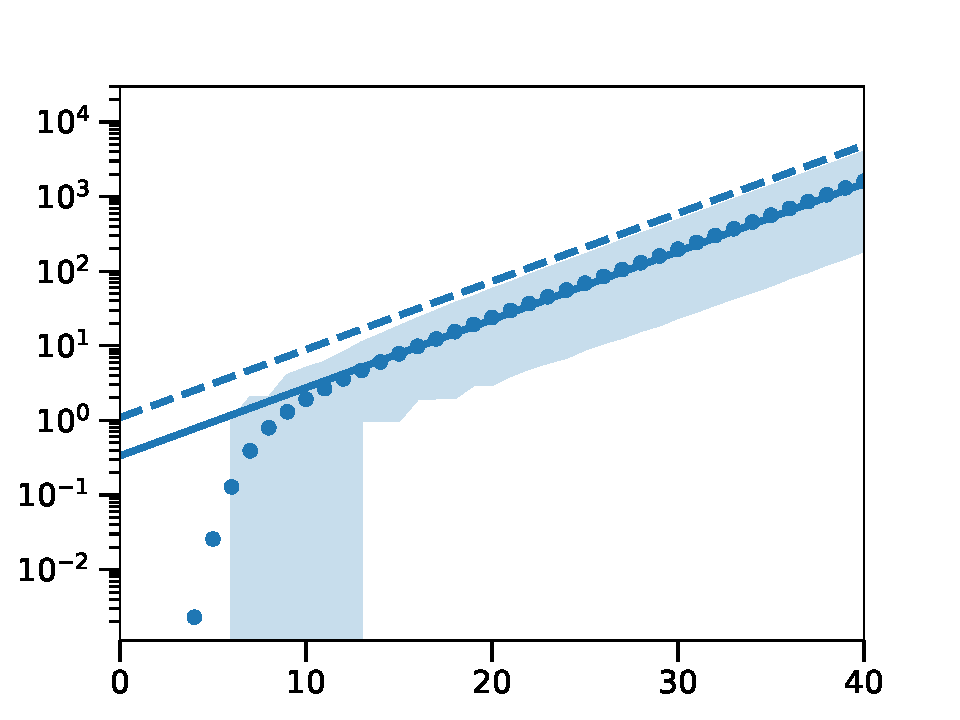
\includegraphics[scale=0.39]{fig3b_blank.pdf}};
   		\begin{scope}[x=(Bild.south east),y=(Bild.north west)]
        	\draw (0.55,-0.035) node {time $t$ [days]};
        	\draw (-0.01,0.5) node [rotate=90] {number of individuals};
        	\draw[thick,color=nb,dashed] (0.15,0.8) -- node[right=6pt] {\color{black} \footnotesize $I_{\text{surv}}(t)$ (Eq. (3))} (0.2,0.8);
        	\draw[thick,color=nb] (0.15,0.71) -- node[right=6pt] {\color{black} \footnotesize $I_{\text{detect}}(t)$ (Eq. (7))} (0.2,0.71);
    		\end{scope}
\end{tikzpicture}

\end{document}